\subsection{Idle Experiment}

During the experiment from \cref{sec:experiment_one}, it was observed that the energy consumption made by the software measuring instruments on the idle experiments was lower than the expectations presented in \cref{subsec:expec_energy_consumption}. An example of this from \cref*{fig:TestCaseIdle_Cores_comparison_energy_without_outliers_avg_watts} is an Intel Power Gadget measurement on the surface pro 4 with a median energy consumption of $1.45W$, where the expectations were between $7.5W and 14W$. Because of this, some further investigation into the results was conducted. In terms of why the measurements were so low, a few things could have caused it, which will be covered now.


            \begin{figure}
                \centering
                \begin{tikzpicture}
                    \pgfplotsset{%
                        width=1\textwidth,
                        height=0.5\textheight
                    }
                    \begin{axis}[
                        xlabel={Start temperature},
                        ylabel={Average dynamic energy (watt)},
                    ]
                    
                    \end{axis}
                \end{tikzpicture} 
            \caption{A graph illustrating the energy consumption of Cores for test case TestCaseIdle with regards to the temperature of the DUT} \label{fig:TestCaseIdle_Cores}
            \end{figure}
            

\paragraph{Implementation:} The original idle test case, was implemented using \texttt{Thread.Sleep()}, so we tried replacing this part of the test case with \texttt{Task.Delay()} to see if this had an impact. The results from this were identical to the previous results, so we ruled out problems with the test case itself.

\paragraph{CPU-states:} Another thing able to cause this, was on the hardware side. In the work by Fahad et al.\cite*[]{fahad2019comparative} they experimented with disabling Core-states (C-states). These states include performance states (P-states) and C-states\cite[]{PCStat}, where the P-states provide a way to change the frequency and voltage of the CPU. Here P0 represents max performance and higher values of P underclock the CPU. The C-states become relevant when the CPU is doing little to no work, where certain parts of the CPU will be turned off, resulting in reduced power consumption. When considering the intuition, purpose and function of the different Power States, it shows that they can drastically affect the power consumption of the DUT and could, depending on the circumstances, change the outcome of the experiments. This would cause the results of the experiments to be incorrect if the Power-States are not in the same state during all test cases. What will be presented here is largely based on information from Intel\cite{CIntel} and some sources that convey the material in a more presentable manner \cite{CMete,CLinux}. The C-states manage how the system consumes energy, C0 is the normal operation of a working computer under load. Each incremental C-State shuts more of the CPU down until at C10 it is nearly completely shut down. Different CPUs and motherboards could however support a different amount of c-states. The same idea applies to CC-States(Core C-states), PC-States(Package C-States) in addition to the Thread C-States and Hyper-Thread C-States, but the information on these is very sparse. Some CPUs also have enhanced C-States (C1E) able to shut more of the CPU down, but not enough to be the next C-State. The P-States are only used during C0, where they control the frequency of the CPU under load to better manage its energy usage. S-States (Sleep State) controls how the system is using energy, but on a larger scale as it controls if the system is sleeping or not. Every C-States occur within S0, while increments define deeper states of sleep such as Sleep and Hibernation. The G-States (Global-States) define the overall state of the system such as G0 being a working computer where S0, C-States and P-States can occur and G3 when the DUT is completely shut down. The expectation based on this is that since the problem only seemed to occur during the idle experiments we suspected it had something to do with the C-states.

\paragraph{C-States:} To test whether the C-states were causing low energy consumption, we tried to disable them in the BIOS. This was only possible on the workstation as the Surface devices had very limited options available. Running the experiments again with the C-states disable seemed to have little to no effect on the measurements. Looking more into the BIOS we discovered that the TUF B360M-PLUS GAMING motherboard had three modes, performance mode, Max power saving mode and automatic. Max power and performance mode would each change multiple BIOS settings where automatic would switch between performance and max power mode. The reason why just disabling the C-states did not impact the results, might be because of this. The specific changes made by max power and performance mode can be seen in \cref{tab:BIOSOptions}.\todo[]{Create graphs illustrating this (results from idlecstatesdisabled)}

\begin{table}[]
    \centering
    \begin{tabular}{|l|l|l|l|}
    \hline
                                                                                   & \begin{tabular}[c]{@{}l@{}}Performance\\  Mode\end{tabular} & \begin{tabular}[c]{@{}l@{}}Max Power-\\ Saving Mode\end{tabular} & Default (Auto) \\ \hline
    Intell(R) SpeedStep                                                            & Disabled                                                    & Enabled                                                          & Auto           \\ \hline
    \begin{tabular}[c]{@{}l@{}}Long Duration \\ Package Power Limit\end{tabular}   & 4095                                                        & Auto                                                             & Auto           \\ \hline
    \begin{tabular}[c]{@{}l@{}}Package Power\\ Time Window\end{tabular}            & 127                                                         & Auto                                                             & Auto           \\ \hline
    Short Duration Power Limit                                                     & 4095                                                        & Auto                                                             & Auto           \\ \hline
    \begin{tabular}[c]{@{}l@{}}CPU Core/Cache\\ Current Limit\end{tabular}         & 255.50                                                      & Auto                                                             & Auto           \\ \hline
    \begin{tabular}[c]{@{}l@{}}PCI Express-\\ Native Power Management\end{tabular} & 255.50                                                      & Enabled                                                          & 255.50         \\ \hline
    Native ASPM                                                                    & Disabled                                                    & Enabled                                                          & Disabled       \\ \hline
    PCH DMI ASPM                                                                   & Disabled                                                    & L0sL1                                                            & Disabled       \\ \hline
    ASPM                                                                           & Disabled                                                    & L0sL1                                                            & Disabled       \\ \hline
    DMI Link ASPM Control                                                          & Disabled                                                    & L0sL1                                                            & Disabled       \\ \hline
    PEG - ASPM                                                                     & Disabled                                                    & ASPM L0sL1                                                       & Disabled       \\ \hline
    \begin{tabular}[c]{@{}l@{}}Intel(R) Speed-\\ Shift Technology\end{tabular}     & Disabled                                                    & Enabled                                                          & Enabled        \\ \hline
    CPU C-states                                                                   & Disabled                                                    & Enabled                                                          & Auto           \\ \hline
    Package C State Limit                                                          & CO/C1                                                       & C10                                                              & C10            \\ \hline
    RC6(Render Standby)                                                            & Disabled                                                    & Enabeld                                                          & Auto           \\ \hline
    Aggressive LPM support                                                         & Disabled                                                    & Enabled                                                          & Enabled        \\ \hline
    \end{tabular}
    \caption{These are the different BIOS setting that change based on which Performance mode is selected}
    \label{tab:BIOSOptions}
\end{table}

\paragraph{Performance mode:} Enabling Performance mode made the idle test case results much more in line with the expectations. Based on this, it seems like during the idle test case the DUT would enter a C-State where it became difficult to measure its energy usage. Initially, we thought that this might affect the software measurements as they were somehow getting slower together with the rest of the CPU and thus taking fewer measurements than expected, causing our calculations to be wrong. To test this hypothesis the idle experiments were run again in performance mode while making hardware measurements. 

\paragraph{Conclusion:} We expected that performance mode would have a negligible effect on the hardware measurements, but the results were an increased energy consumption for both hardware and software measuring instruments. This seems to indicate that the power saving ability of the various C-States built into the motherboard and CPU is much more impactful than expected. Given that the C-States drastically influenced how the DUT uses energy, and that they would ideally not be entered during any of the other test cases, it makes sense to disable the C-states so none of the test cases is using them. Furthermore, the purpose of this study is to compare the measuring instruments and not the measurements themselves. Some sources mention it might be possible to control the C-states through the OS\cite{CMete,CLinux}, but due to time constraints, this was not explored any further and was only done on the workstation, where the C-states could be changed through the BIOS. Given that it is only the workstation that can disable the C-States a second experiment will be conducted with the C-states disabled for this DUT only.